% 元の
% \documentclass[lualatex,book,paper=a4paper,jafontsize=11.5pt,jafontscale=1.05]{jlreq}
\documentclass[lualatex,paper=a4paper,jafontsize=11.5pt,jafontscale=1.05]{jlreq}
% 2ページ目や章の前に一ページ余分なものがあるのが気になる場合は openanyを\documentclass[...,book,openany ,..]として追加する

%フォント:
\usepackage{luatexja-fontspec}
\usepackage{hack-fonts}

%表紙用:
\usepackage{hack-cover}
\usepackage{enumitem}
% 画像
\usepackage{graphicx}
\usepackage{float}

% リンク
\usepackage[hidelinks]{hyperref}

% ソースコード
\usepackage{listings}
\lstset{
  frame=single,
  basicstyle=\small\ttfamily,
  tabsize=4,
  breaklines=true
}

% 色・ガントチャート
\usepackage{xcolor}
\usepackage{pgfgantt}
\usepackage{caption}

\begin{document}
\section*{作業ログ}
\noindent
報告者:恩田 隼士\\
報告日: \today \\
プロジェクト名: 単一のフルカラーLEDとArduinoを用いた光無線通信による楽器間同期演奏システム \\
\hrulefill

\section{進捗サマリー（概要）}
\begin{itemize}
 \item 全体進捗率: 80\%
 \item マイルストーン達成状況: 達成
 \item 主要成果:
 \begin{itemize}
    \item ヴァイオリン音のスペクトラム分析・波形合成（完了・進捗100\%）
    \item 演奏開始・停止スイッチの実装（完了・進捗100\%）
    \item ヴァイオリン音・開始停止スイッチの単体動作テスト（完了）
    \item 40倍音までのスペクトル分析に基づく倍音調整により，実楽器に近いヴァイオリン音を再現できた．
 \end{itemize}
 \item 重大課題（影響度）: なし
\end{itemize}

\section{作業ログ（詳細トラッキング）}
\begin{table}[H]
  \centering
  \caption{作業ログ}
   \scalebox{0.7}{
    \begin{tabular}{lcccccc} \hline
      作業項目 & 開始日 & 予定完了日 & 状態 & 進捗率 & 依存関係・ブロッカー & コメント \\ \hline
      楽器演奏 & 05/20 & 05/23 & 完了 & 100\% & なし & - \\
      演奏開始・停止ボタン（設計） & 05/23 & 05/27 & 完了 & 100\% & 部品入手 & - \\
      楽器音 & 05/23 & 05/27 & 完了 & 100\% & 楽器演奏 & - \\
      楽譜配列 & 05/26 & 05/28 & 完了 & 100\% & 楽器音 & - \\
      ヴァイオリン音 & 05/28 & 06/12 & 完了 & 100\% & 楽器音 & 今週完了 \\
      演奏開始・停止ボタン（実装） & 05/28 & 06/09 & 完了 & 100\% & 設計 & - \\
      開始停止スイッチテスト & 06/13 & 06/19 & 進行中 & 50\% & 実装の完了 & 単体は確認済，結合は他担当待ち \\
      楽器音テスト & 06/13 & 06/19 & 進行中 & 50\% & 実装の完了 & 単体は確認済，結合は他担当待ち \\
      \hline
    \end{tabular}
  }
\end{table}


% ===== 計画前ガントチャート =====
\subsection{担当箇所のガントチャート（計画前）}
\noindent
\begin{figure}[H]
\centering
\resizebox{0.92\linewidth}{!}{%
\begin{ganttchart}[
  hgrid,
  vgrid={*6{draw=none,line width=0pt}, dotted},
  time slot format=isodate,
  time slot unit=day,
  x unit=0.52cm,
  y unit title=0.6cm,
  y unit chart=0.65cm,
  title label font=\tiny,
  bar label font=\small,
  bar label node/.append style={text width=4.8cm, align=right},
  bar height=0.55,
  bar top shift=0.23,
  bar/.append style={fill=violet!45, draw=violet!75},
]{2026-05-20}{2026-06-16}
  \gantttitlecalendar{month=shortname, day} \\
  \ganttbar{楽器演奏}{2026-05-20}{2026-05-23} \\
  \ganttbar{演奏開始・停止ボタン}{2026-05-23}{2026-05-27} \\
  \ganttbar{楽器音}{2026-05-23}{2026-05-27} \\
  \ganttbar{楽譜配列}{2026-05-26}{2026-05-28} \\
  \ganttbar{ヴァイオリン音}{2026-05-28}{2026-05-31}
  \ganttbar[bar label node/.append style={opacity=0}]{}{2026-06-04}{2026-06-09} \\
  \ganttbar{開始停止スイッチテスト}{2026-06-10}{2026-06-16} \\
  \ganttbar{楽器音テスト}{2026-06-10}{2026-06-16}
\end{ganttchart}%
}
\caption{担当箇所ガントチャート（計画前）}
\end{figure}

% ===== 現在のガントチャート =====
% 凡例：■ 灰色 = 完了，■ 紫色 = 未完了 / 進行中
% タスクの状態に応じて fill=gray!60（完了）または fill=violet!50（未完了）を変更
\subsection{担当箇所のガントチャート（現在・進捗状況）}
\noindent
{\small \textcolor{gray!50}{\rule{1em}{0.8em}}\ 完了\quad
       \textcolor{violet!60}{\rule{1em}{0.8em}}\ 未完了／進行中}
\begin{figure}[H]
\centering
\resizebox{0.92\linewidth}{!}{%
\begin{ganttchart}[
  hgrid,
  vgrid={*6{draw=none,line width=0pt}, dotted},
  time slot format=isodate,
  time slot unit=day,
  x unit=0.52cm,
  y unit title=0.6cm,
  y unit chart=0.65cm,
  title label font=\tiny,
  bar label font=\small,
  bar label node/.append style={text width=4.8cm, align=right},
  bar height=0.55,
  bar top shift=0.23,
]{2026-05-20}{2026-06-19}
  \gantttitlecalendar{month=shortname, day} \\
  % ---- 完了タスク (gray!60) ----
  \ganttbar[bar/.append style={fill=gray!60, draw=gray!80}]
    {楽器演奏}{2026-05-20}{2026-05-23} \\
  \ganttbar[bar/.append style={fill=gray!60, draw=gray!80}]
    {演奏開始・停止ボタン（設計）}{2026-05-23}{2026-05-27} \\
  \ganttbar[bar/.append style={fill=gray!60, draw=gray!80}]
    {楽器音}{2026-05-23}{2026-05-27} \\
  \ganttbar[bar/.append style={fill=gray!60, draw=gray!80}]
    {楽譜配列}{2026-05-26}{2026-05-28} \\
  % ---- ヴァイオリン音：今週完了 (gray!60) ----
  \ganttbar[bar/.append style={fill=gray!60, draw=gray!80}]
    {ヴァイオリン音}{2026-05-28}{2026-05-31}
  \ganttbar[bar/.append style={fill=gray!60, draw=gray!80},
    bar label node/.append style={opacity=0}]
    {}{2026-06-04}{2026-06-12} \\
  \ganttbar[bar/.append style={fill=gray!60, draw=gray!80}]
    {演奏開始・停止ボタン（実装）}{2026-05-28}{2026-05-31}
  \ganttbar[bar/.append style={fill=gray!60, draw=gray!80},
    bar label node/.append style={opacity=0}]
    {}{2026-06-04}{2026-06-09} \\
  % ---- 進行中タスク (violet!50)：単体確認済・結合は他担当待ち ----
  \ganttbar[bar/.append style={fill=violet!50, draw=violet!80}]
    {開始停止スイッチテスト}{2026-06-13}{2026-06-19} \\
  \ganttbar[bar/.append style={fill=violet!50, draw=violet!80}]
    {楽器音テスト}{2026-06-13}{2026-06-19}
\end{ganttchart}%
}
\caption{担当箇所ガントチャート（現在：灰＝完了，紫＝未完了）}
\end{figure}

ガントチャートにおいて，06/01$\sim$06/03の期間はテスト期間として空白にしている．

% ===== 日ごとの作業時間・内容 =====
\subsection{日ごとの作業時間・内容}
\begin{table}[H]
  \centering
  \caption{日ごとの作業時間・内容}
  \scalebox{0.88}{
    \begin{tabular}{ccp{7.5cm}} \hline
      日付 & 作業時間 & 作業内容・備考 \\ \hline
      2026/06/10 & 4h & ヴァイオリン音・開始停止スイッチの単体動作テスト \\[4pt]
      2026/06/16 & 4h & ヴァイオリン音の倍音調整（40倍音まで）・音色再現性テスト \\[4pt]
        % ※必要に応じて行を追加
      \hline
    \end{tabular}
  }

\end{table}

% ===== 今週追加：ログの詳細（TPM・TRL） =====
\section{ログの詳細}

\subsection{ヴァイオリン音再現の詳細}
目標とする実ヴァイオリン音と，本システムの生成波形のそれぞれにスペクトル分析を行い，
各倍音の大きさを読み取った．再現性を高めるため40倍音までの振幅を計測し，
それに合わせて倍音を調整することで，実楽器に近いヴァイオリン音を近似できた．
なお，比較にあたっては各音を基準音と音量正規化・音程確認した上で行っており，
音程のずれは知覚上許容される範囲に収まることを確認した\cite{Vurma}．
評価結果を図\ref{fig:violin_result}に示す．
\begin{figure}[H]
  \centering
  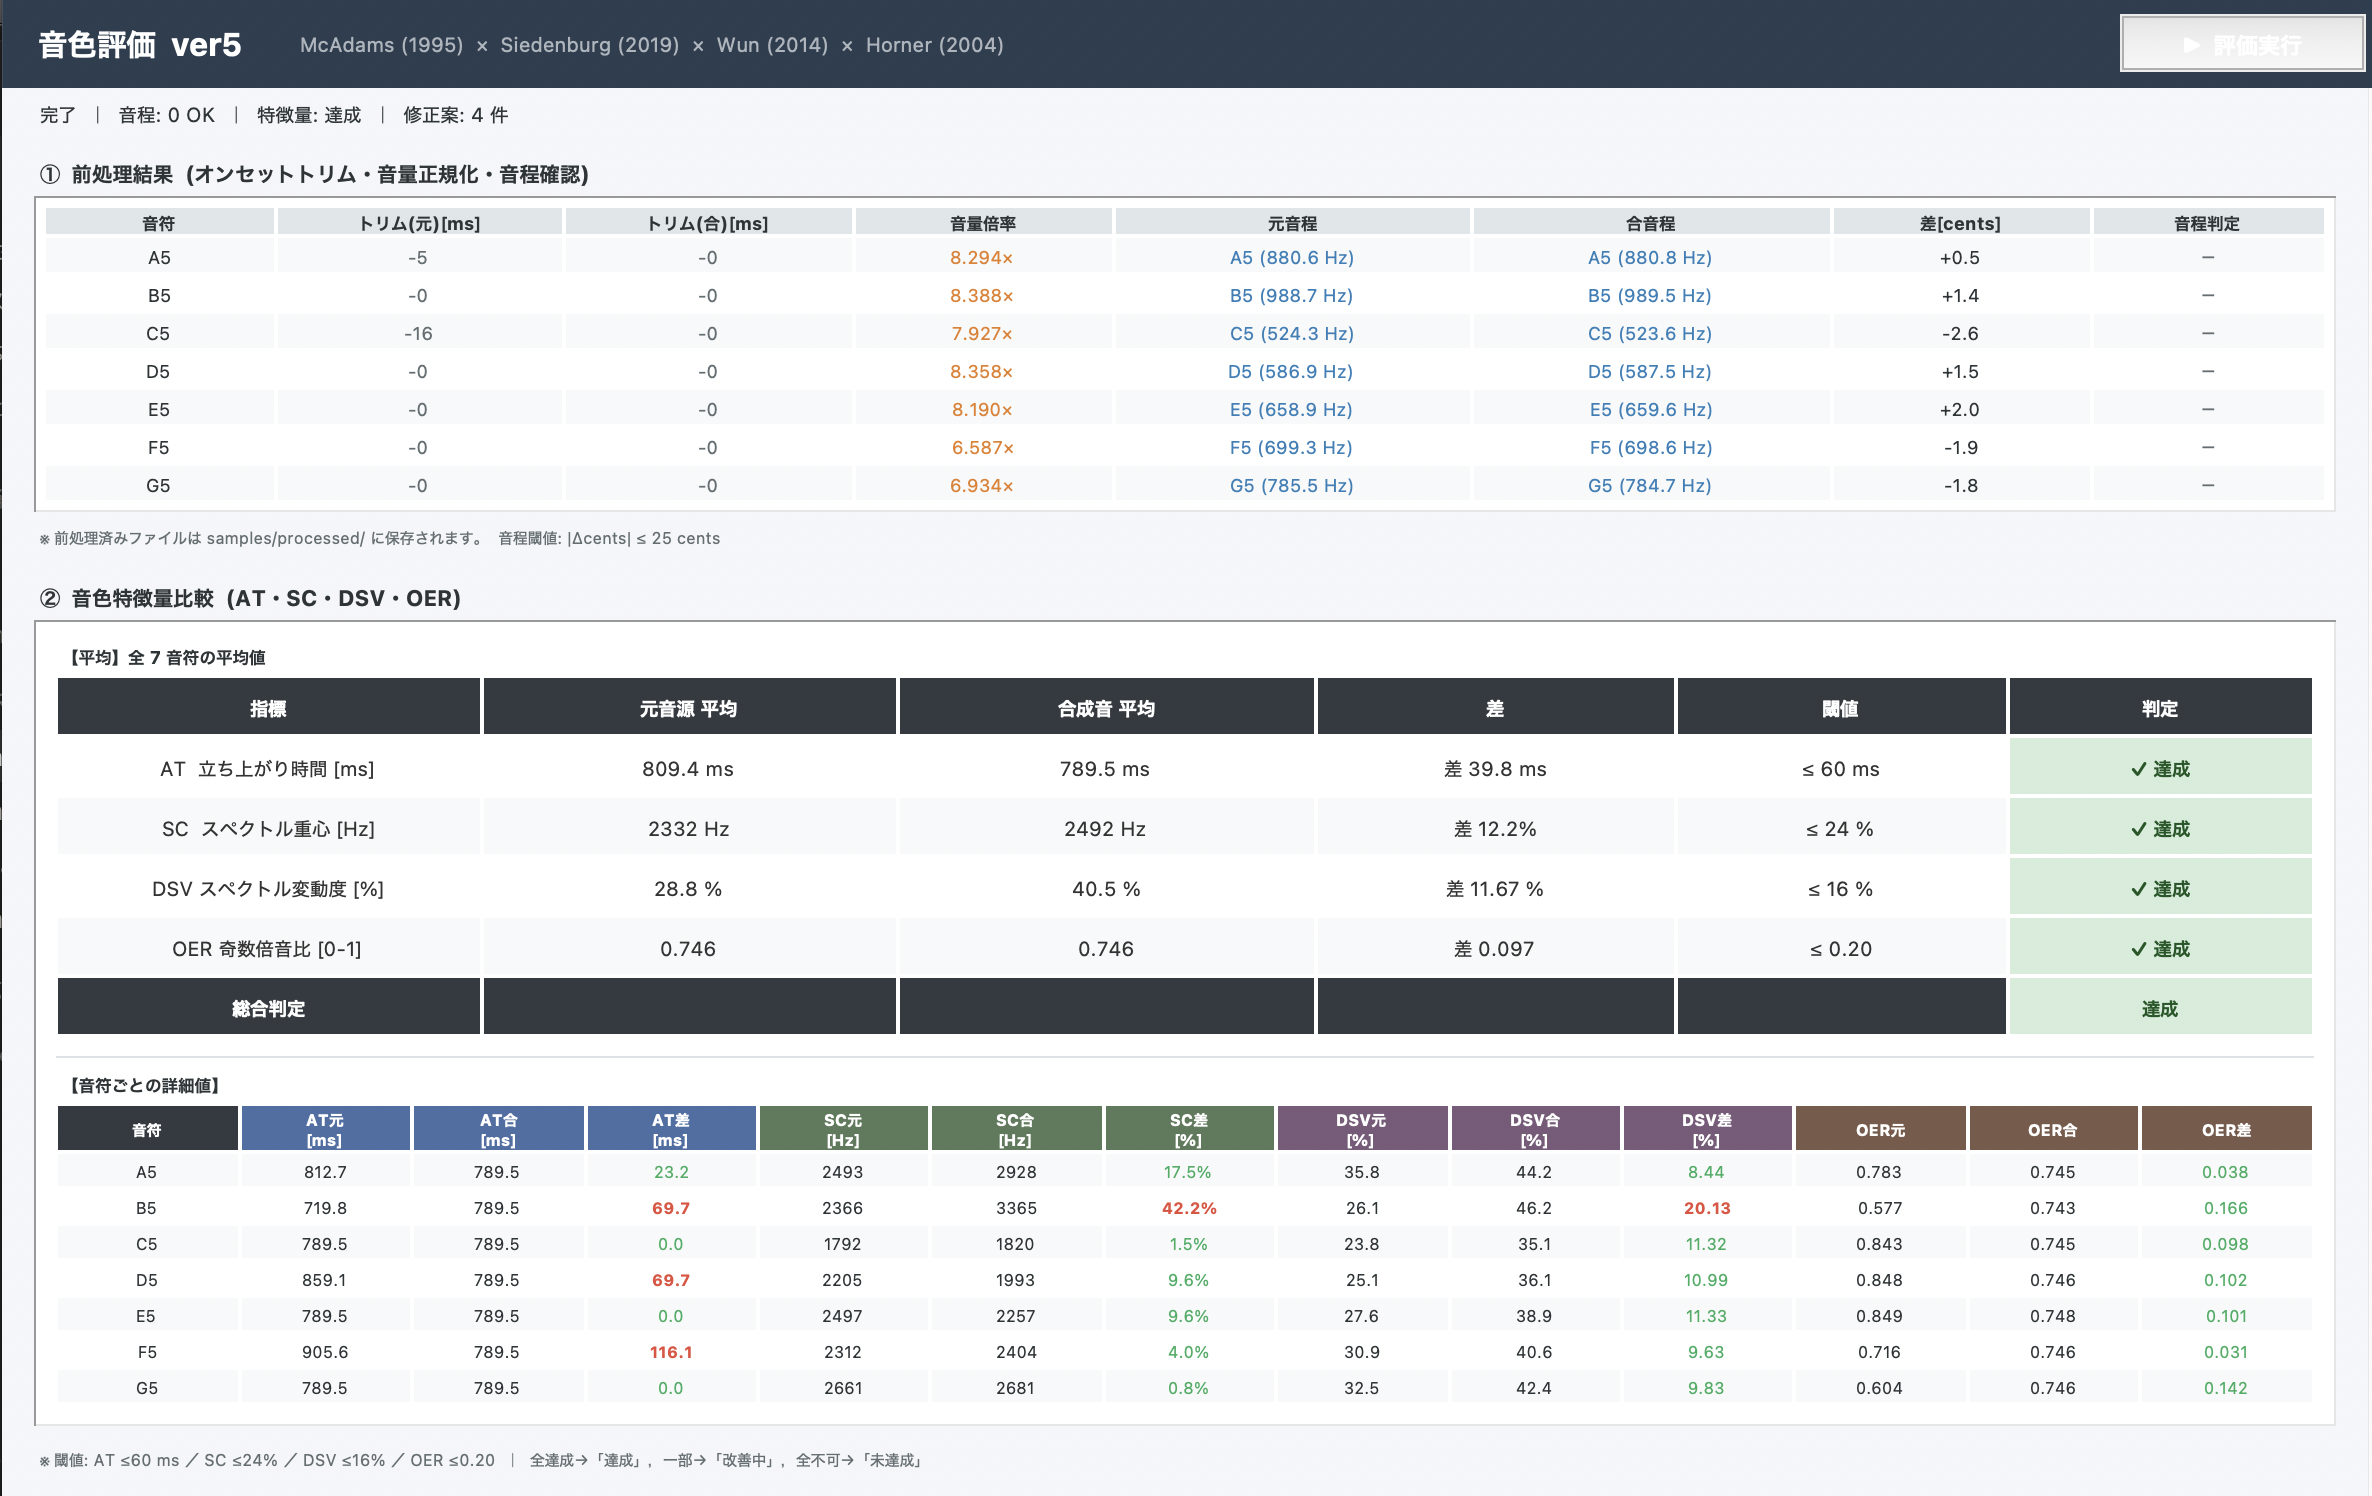
\includegraphics[width=0.95\linewidth]{violin_result.png}
  \caption{ヴァイオリン音の音色評価結果（音色特徴量比較）}
  \label{fig:violin_result}
\end{figure}

\subsection{技術性能指標（TPM）}
TPMはシステムの最終的な性能に関わる技術を管理するための指標である．
本プロジェクトの各指標のうち，自分の担当は「音色の再現性」である．
実楽器音の録音と本システムの出力音を比較する．演奏の正確性（accuracy）は
一意に定義することが難しいため\cite{Larrouy}，本テストでは人間の音色知覚を構成する
以下の4特徴量を定量指標として再現精度を評価する\cite{McAdams}．各楽器・音程ごとに計測し，平均で評価する．

\begin{itemize}
  \item 立ち上がり時間（AT）：RMSエンベロープがピークに到達するまでの時間[ms]．
        目標は全音程平均で60\,ms以内\cite{Siedenburg}．
  \item スペクトル重心（SC）：持続区間のスペクトル重心周波数[Hz]．
        目標は相対差の平均で24\%以内\cite{Wun}．
  \item スペクトル変動度（DSV）：フレーム間のL2相対変化量の平均[\%]．
        目標はズレの平均で16\%以内\cite{McAdams}．
  \item 奇偶倍音比（OER）：pYINアルゴリズムでF0を推定し，奇数次倍音と
        全倍音のエネルギー比を算出．目標は相対差の平均で20\%以内\cite{Caclin}．
\end{itemize}

今週の計測結果（全7音程の平均）を表\ref{tab:tpm}に示す．いずれの特徴量も目標値を満たし，
担当指標である音色の再現性は達成と判定した（詳細は図\ref{fig:violin_result}）．

\begin{table}[H]
  \centering
  \caption{音色の再現性（TPM）計測結果}
  \label{tab:tpm}
  \scalebox{0.9}{
    \begin{tabular}{lcccc} \hline
      特徴量 & 元音平均 & 合成音平均 & 差（目標） & 判定 \\ \hline
      AT [ms]  & 809.4 & 769.5 & 39.6\,ms（$\leq$60\,ms） & 達成 \\
      SC [Hz]  & 2332  & 2492  & 12.2\%（$\leq$24\%） & 達成 \\
      DSV [\%] & 28.6  & 40.5  & 11.67\%（$\leq$16\%） & 達成 \\
      OER [0--1] & 0.746 & 0.746 & 0.097（$\leq$0.20） & 達成 \\
      \hline
    \end{tabular}
  }
\end{table}

\subsection{技術成熟度（TRL）}
TRLは機能ごとの進捗を確認する指標である．定義を表\ref{tab:trl}に示す．

\begin{table}[H]
  \centering
  \caption{TRLの定義}
  \label{tab:trl}
  \scalebox{0.9}{
    \begin{tabular}{cp{10cm}} \hline
      TRL & 定義 \\ \hline
      1 & 概念レベル：アイディアや原理が確立されており，説明できるレベル \\
      2 & 基本動作レベル：単体で動作確認が可能なレベル \\
      3 & 結合動作レベル：機能を結合し，実際の使用環境に近い環境で動作確認が可能なレベル \\
      4 & 実運用レベル：実際の使用環境で安定的な稼働が確認できるレベル \\
      \hline
    \end{tabular}
  }
\end{table}

自分の担当機能の現状を表\ref{tab:trl_status}に示す．ヴァイオリン音生成・開始停止スイッチは
いずれも単体での動作確認が完了しているためTRL2に到達している．
機能を結合した結合テストは他担当の実装待ちであり，TRL3には未到達である．

\begin{table}[H]
  \centering
  \caption{担当機能のTRL現状}
  \label{tab:trl_status}
  \scalebox{0.9}{
    \begin{tabular}{lcp{6cm}} \hline
      担当機能 & 現在のTRL & 根拠 \\ \hline
      ヴァイオリン音生成 & TRL2 & 単体で目標音色を再現・計測済み．結合は他担当待ち \\
      開始停止スイッチ & TRL2 & 単体で開始・停止動作を確認済み．結合は他担当待ち \\
      \hline
    \end{tabular}
  }
\end{table}

\section{課題管理}

\subsection{コード統合}
\begin{itemize}
  \item 原因: 各担当者が個別に実装を進めているため，統合時にコードの調整が必要となる．
  \item 影響度: 中
  \item 優先度: 中
  \item 対応策: 他担当者と実装の仕様・コードを確認し，統合作業を計画的に進める．
  \item 期限: 2026/06/19
  \item 状態: 未着手
\end{itemize}


% ※影響度＝プロジェクトへのインパクト
% ※優先度＝対応の緊急性

\section{AI利用状況と検証}
\subsection{利用内容：合成波形の自動録音プログラム}
\begin{itemize}
    \item 利用目的：楽器音単体テストに使用する音源の実装
    \item 入力（プロンプト要旨）：
    \begin{itemize}
        \item Processingで合成した波形音を一音ずつ自動で録音するプログラムの作成を依頼した．
        \item 既存の波形生成pdeとは別ファイルとし，波形の内容（合成方法・倍音構成）は同一とする旨を指定した．
        \item 立ち上がり（noteOn）から1秒間鳴らし，C5〜B5の白鍵7音（\texttt{C5 D5 E5 F5 G5 A5 B5}）を1音ずつ録音すること，および録音時間をコード内の定数で変更できる構造にすることを指定した．
        \item 録音時に必ずしも音をスピーカから出力する必要はない旨を指定した．
    \end{itemize}
    \item 出力概要：
    \begin{itemize}
        \item 録音仕様：C5〜B5の白鍵7音を1音ずつ自動で \texttt{recordings/C5.wav} 〜 \texttt{recordings/B5.wav} に保存する実装が得られた．
        \item 録音タイミング：noteOnから \texttt{RECORD\_SECONDS} 秒間を録音し，1音終わると即 \texttt{doUnpatch()}（\texttt{violin.pde} 内で定義した自作ヘルパー関数．内部で各倍音 \texttt{UGen} に対して Minim の \texttt{unpatch()}\cite{minim_unpatch} を呼び出し，出力との接続を解除するラッパー）で停止．\texttt{GAP\_SECONDS} の無音区間を挟んで次の音へ遷移する制御が得られた．
        \item 録音時間の変更：コード冒頭の定数 \texttt{final float RECORD\_SECONDS = 1.0;} を書き換えることで，任意の録音長に変更可能である．
        \item 音出力について：Minimの \texttt{AudioRecorder} はラインアウトを録音する仕組みのため，実行中はスピーカからも音が鳴る（録音自体に再生は必須ではないという条件は満たす．気になる場合はシステム音量を下げてもファイルには影響しない）旨の補足が得られた．
    \end{itemize}
\end{itemize}

\subsection{検証方法}
% ※第三者が再現できるレベルで記述
\begin{itemize}
  \item 検証方法:
  \begin{itemize}
      \item 実機での実行による動作確認，および生成されたwavファイルの再生確認．
  \end{itemize}
  \item 参照資料:
  \begin{itemize}
      \item Processing公式リファレンス\cite{processing}．
  \end{itemize}
  \item 検証手順：
  \begin{enumerate}
      \item 録音プログラム（pde）を実行し，実行時にエラーが発生しないことを確認する．
      \item \texttt{recordings/} ディレクトリ配下にC5〜B5の白鍵7音分のwavファイルが生成されていることを確認する．
      \item 生成されたwavファイルを再生し，意図した波形音が正しく録音されていることを確認する．
  \end{enumerate}
\end{itemize}

\subsection{ファクトチェック}
\begin{itemize}
  \item 一致点：
  \begin{itemize}
    \item AIが提示した実装方法（Minimの\texttt{AudioRecorder}による録音，および自作ヘルパー \texttt{doUnpatch()} を介した Minim \texttt{UGen.unpatch()}\cite{minim_unpatch} による発音停止）は，Processing公式リファレンス\cite{processing}およびMinim公式ドキュメントの記載と一致する．
  \end{itemize}
  \item 不一致・疑義：なし
  \item 最終判断：採用
  \item 根拠：
  \begin{itemize}
    \item 生成されたwavファイルと，元の波形生成pdeから出力される音源とを聴感上で比較し，差異がないことを確認した．
  \end{itemize}
\end{itemize}

\section{次回計画（次回までに実施する内容）}
\begin{itemize}
  \item 実施事項：結合テスト（他担当との統合）
  \begin{itemize}
    \item 他担当の実装完了後，ヴァイオリン音・開始停止スイッチを結合し，実使用環境に近い条件で動作テストを実施する（TRL3を目指す）．
  \end{itemize}
  \item 達成基準：
  \begin{itemize}
    \item 結合状態で演奏の開始・停止および各音の発音が正しく動作すること．
  \end{itemize}
  \item 期限：2026/06/19
\end{itemize}

\section{その他}
連絡事項・懸念点：なし

\section{付録}
添付資料を以下のリポジトリURLに示す．添付範囲は全体である．\\
\url{https://github.com/crab2424/LEDplaying_system}



\begin{thebibliography}{9}
\bibitem{processing} Processing Foundation (2026), "Processing Reference". \url{https://processing.org/reference/}. (2026年6月16日 参照)
\bibitem{minim_unpatch} D. Di Fede (2026), "Minim : UGen.unpatch()". \url{http://code.compartmental.net/minim/ugen_method_unpatch.html}. (2026年6月16日 参照)
\bibitem{Vurma} A. Vurma and J. Ross, "Production and perception of musical intervals," \textit{Music Perception}, vol. 23, no. 4, pp. 331--344, 2006.
\bibitem{Larrouy} P. Larrouy-Maestri, "I know it when I hear it," \textit{Music \& Science}, vol. 1, 2018.
\bibitem{McAdams} S. McAdams, S. Winsberg, S. Donnadieu, G. De Soete, and J. Krimphoff, "Perceptual scaling of synthesized musical timbres: Common dimensions, specificities, and latent subject classes," \textit{Psychological Research}, vol. 58, no. 3, pp. 177--192, 1995.
\bibitem{Caclin} A. Caclin, S. McAdams, B. K. Smith, and S. Winsberg, "Acoustic correlates of timbre space dimensions: A confirmatory study using synthetic tones," \textit{The Journal of the Acoustical Society of America}, vol. 118, no. 1, pp. 471--482, 2005.
\bibitem{Siedenburg} K. Siedenburg, "Specifying the perceptual relevance of onset transients for musical instrument identification," \textit{The Journal of the Acoustical Society of America}, vol. 145, no. 2, pp. 1078--1087, 2019.
\bibitem{Wun} S. Wun, A. Horner, and B. Wu, "Effect of spectral centroid manipulation on discrimination and identification of instrument timbres," \textit{Journal of the Audio Engineering Society}, vol. 62, no. 9, pp. 575--583, 2014.
\end{thebibliography}

\end{document}
